%&tex

\documentclass[tikz,margin=2mm]{standalone}
\usetikzlibrary{calc}
\tikzset{
  dim above/.style={to path={\pgfextra{
        \pgfinterruptpath
        \draw[line width=.4pt,>=latex,|<->|] let
        \p1=($(\tikztostart)!2mm!90:(\tikztotarget)$),
        \p2=($(\tikztotarget)!2mm!-90:(\tikztostart)$)
        in (\p1) -- (\p2) node[text=,pos=.5,sloped,above]{#1};
        \endpgfinterruptpath
      } -- (\tikztotarget) \tikztonodes
    }
  },
  dim below/.style={to path={\pgfextra{
        \pgfinterruptpath
        \draw[line width=.4pt,>=latex,|<->|] let
        \p1=($(\tikztostart)!-3mm!90:(\tikztotarget)$),
        \p2=($(\tikztotarget)!-3mm!-90:(\tikztostart)$)
        in (\p1) -- (\p2) node[text=,pos=.5,sloped,below]{#1};
        \endpgfinterruptpath
      } -- (\tikztotarget) \tikztonodes
    }
  }
}

\begin{document}
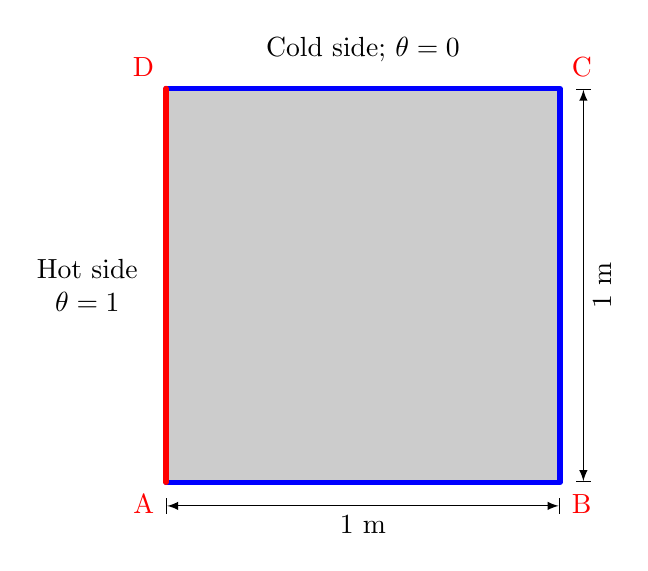
\begin{tikzpicture}
    \path[draw = blue, text = red, line width=2pt, fill = black!20, line cap = round, line join = round]
    (0,0)
    to [dim below = 1 m] (5,0) node[below right] {B}
    to [dim below = 1 m] (5,5) node[above right] {C}
    to (0,5) node[above left] {D};
    \path[draw = red, text = red, line width=2pt, fill = black!20, line cap = round, line join = round]
    (0,5)
    to (0,0) node[below left] {A};

    \node[minimum size=1cm,label={[align=center]center:Hot side \\ \(\theta = 1\)}] at (-1,2.5) {};
    \node[label = {[align=center]center:Cold side; \(\theta = 0\)}] at (2.5,5.5) {};
\end{tikzpicture}
\end{document}
